% LTeX: language=en-GB enabled=false

\documentclass[10pt]{article}
\usepackage[utf8]{inputenc}
\usepackage{amsmath, amssymb, amsthm, physics, listings}
\usepackage[T1]{fontenc}
\usepackage{microtype}
\usepackage{graphicx, float, xcolor, tikz, pgfplots, pgfplotstable, tikz-3dplot}
\usepackage[inline]{asymptote}

\pgfplotsset{compat=1.18}
\usetikzlibrary{patterns, angles, quotes}

\usepackage[backend=biber, style=numeric, language=british,sorting=none]{biblatex}
\addbibresource{references.bib}

\usepackage[a4paper, top=1in, bottom=1in, left=1in, right=1in, heightrounded]{geometry}
\renewcommand{\baselinestretch}{1.15}
\setlength{\parindent}{0pt}
\setlength{\parskip}{0.8em}

\renewcommand{\thefootnote}{\fnsymbol{footnote}}
\setlength{\skip\footins}{1cm}

\title{The use of quaternions in the computation of 3D rotations}
\author{Shayan Nezami}
\date{\today}

% LTeX: language=en-GB enabled=true

\begin{document}

\maketitle
\vspace{10pt}
\tableofcontents
\pagebreak

\section{Introduction}

\subsection{What are quaternions?}

Quaternions are a 4-dimensional number system that extend the complex numbers, in a similar way that the complex numbers extend the real numbers. Denoted $\mathbb{H}$, they are of the form:
\begin{equation}
    a + b\vb{i} + c\vb{j} + d\vb{k}, \quad a, b, c, d \in \mathbb{R}, \quad \vb{i}^2=\vb{j}^2=\vb{k}^2=-1.
\end{equation}
The first term is referred to as the real part of the quaternion, while the other three components are imaginary. Each of these components (which can be thought of as axes in a 4-dimensional space) are orthogonal (perpendicular), and as such no real transformation on any component can map it onto another.

In the modern day, they are used extensively in representing the rotations of 3-dimensional objects in computer systems, due to the relative computational ease of calculating such rotations, which only involves the addition and multiplication of real numbers, and so is much more computationally efficient than other methods of calculating rotation, such as Euler angles, which are perhaps easier to visualise and more widely used outside computational settings. \cite{QuaternionWiki}

\subsection{The structure of this essay}

After this brief introduction, some widely used key terms relating to quaternions will be defined, which will be essential to understanding the following chapters. Next, the additive and (more importantly) multiplicative properties of quaternions will be covered, which in effect govern how they are able to represent 3D rotations, and here the definition of - and need for - the quaternion number system will be derived.

Having covered these areas, the mechanism in which they can be used for rotations will be discussed in depth, including relevant proofs and how to construct rotations with quaternions. The essay will conclude by discussing the applications and desirable properties of quaternions.

The main body of the essay, where most of the explanations are, after the key definitions and properties are stated, starts from Section \ref{ijkComponentsSection}, on page \pageref{ijkComponentsSection}, although the sections on conjugate quaternions and the commutativity of quaternion multiplication are particularly important (Sections \ref{qBarDef} and \ref{ComAss} respectively).

Wherever any information, or inspiration, is taken from a source, it is cited in square brackets, with the numbers corresponding to the bibliography entries. All explanations and diagrams that are not followed by a citation are my original work.

This essay has been written with \LaTeX{} using the VimTeX plugin. Figure \ref{ComplexRotationFig} has been created with GeoGebra and Asymptote, while all of the other Figures have been made with TikZ.

\subsection{Definitions}

\subsubsection{Pure quaternions} \label{PureDef}

A pure quaternion is a quaternion that has no real component, meaning for a quaternion $a + b\vb{i} + c\vb{j} + d\vb{k}$, $a = 0$. \cite{Math431}

They are also known as vector quaternions, as pure quaternions can be used to represent vectors in quaternion form, where the $\vb{i, j}$, and $\vb{k}$ components of the quaternion represent the $x, y$, and $z$ components of a vector respectively.

For example, the vector $(2,3,1)$ can be represented as the quaternion $2\vb{i} + 3\vb{j} + \vb{k}$.

\subsubsection{Unit quaternions}

A unit quaternion is a quaternion with norm 1, i.e: $\abs{q} = 1$ for a quaternion, $q$. \cite{DRose}

\subsubsection{The norm of a quaternion}

The norm, $\abs{q}$, of a quaternion, $q$, is defined as:
\begin{equation}
    \begin{aligned}
        &\abs{q} = \sqrt{a^2 + b^2 + c^2 + d^2}, \\
        \text{where } & q = a + b\vb{i} + c\vb{j} + d\vb{k}.
    \end{aligned} 
\end{equation}
This could be thought of as similar to the magnitude of a vector, giving the theoretical "length" of the quaternion. \cite{Math431}

This is referred to as the norm, as it is what each component of a quaternion needs to be divided by to normalise it (to get its corresponding unit quaternion - one with the same theoretical "direction").

For example, to normalise the quaternion
\begin{equation}
    q = 2 + 3\vb{i} - 4\vb{j} + 5\vb{k},
\end{equation}
one would first find its norm:
\begin{equation}
    \abs{q} = \sqrt{2^2 + 3^2 + (-4)^2 + 5^2} = 3\sqrt{6},
\end{equation}
and then divide each of its components by the norm:
\begin{equation}
    q_u = \frac{2}{3\sqrt{6}}+\frac{3}{3\sqrt{6}}\vb{i}+\frac{4}{3\sqrt{6}}\vb{j}+\frac{5}{3\sqrt{6}}\vb{k}.
\end{equation}
It can be proven that this is indeed a unit quaternion, as
\begin{equation}
    \abs{q_u} = \sqrt{\left(\frac{2}{3\sqrt{6}}\right)^2+\left(\frac{3}{3\sqrt{6}}\right)^2+\left(\frac{4}{3\sqrt{6}}\right)^2+\left(\frac{5}{3\sqrt{6}}\right)^2} = 1.
\end{equation}

\subsubsection{The conjugate of a quaternion} \label{qBarDef}

Every quaternion, $q$, has a conjugate, $\bar{q}$, which is defined as: \cite{DRose}
\begin{equation}
    \begin{aligned}
        &\bar{q} = a - b\vb{i} - c\vb{j} - d\vb{k}, \\
        \text{where } & q = a + b\vb{i} + c\vb{j} + d\vb{k}.
    \end{aligned}
\end{equation}

Using the multiplicative rules for quaternions, which will be explained in Section \ref{ijkComponentsSection}, it can be proven that for any unit quaternion $q$, $q\bar{q} = \bar{q}q = 1$:
\begin{equation}
    \begin{aligned}
        q\bar{q} &= (a + b\vb{i} + c\vb{j} + d\vb{k})(a - b\vb{i} - c\vb{j} - d\vb{k}) \\
                 &= a^2 - ab\vb{i} - ac\vb{j} - ad\vb{k} \\
                 &\phantom{= } + ab\vb{i} - b^2\vb{i}^2 - bc\vb{ij} - bd\vb{ik} \\
                 &\phantom{= } + ac\vb{j} - bc\vb{ji} - c^2\vb{j}^2 -cd\vb{jk} \\
                 &\phantom{= } + ad\vb{k} - bd\vb{ki} - cd\vb{kj} - d^2\vb{k}^2 \\
                 &= a^2 + b^2 + c^2 + d^2 \\
                 &\phantom{= } - bc\vb{ij} - bd\vb{ik} - bc\vb{ji} - cd\vb{jk} - bd\vb{ki} - cd\vb{kj} \\
                 &= a^2 + b^2 + c^2 + d^2 \\
                 &\phantom{= } - bc\vb{k} + bd\vb{j} + bc\vb{k} - cd\vb{i} - bd\vb{j} + cd\vb{i} \\
                 &= a^2 + b^2 + c^2 + d^2 = 1, \text{ since $q$ is a unit quaternion}.
    \end{aligned}
\end{equation}

It can be shown that $\bar{q}q = q\bar{q}$, since $\bar{q} = -q + 2a$ (where $a$ is the real component of $q$), so $\bar{q}$ is a real (-1) multiple of $q$ plus a real number ($2a$), meaning that the multiplication of these two quaternions can be considered commutative, producing the same result regardless of order.

\section{Defining Properties of Quaternions}

The algebraic field of quaternions is defined by certain core properties, which are explored below.

The additive properties are mostly included for context and completeness, while the multiplicative properties are essential for the rotation calculations that will follow - it is in effect these multiplicative properties that mean quaternions are able to compute 3D rotation.

Throughout this section it is to be assumed that $q_n \in \mathbb{H}$, and $a_n, b_n, c_n, d_n \in \mathbb{R}$.

\subsection{Additive properties}

\subsubsection{Closure}

Quaternions are considered closed upon addition. This means that:
\begin{equation}
    q_1, q_2 \in \mathbb{H} \implies q_1 + q_2 \in \mathbb{H}.
\end{equation}
In words, the addition of any two quaternions will necessarily produce a quaternion. \cite{Illinois}

\subsubsection{Commutativity and associativity}

Quaternion addition is both commutative,
\begin{equation}
    q_1 + q_2 = q_2 + q_1,
\end{equation}
and associative \cite{Illinois},
\begin{equation}
    (q_1 + q_2) + q_3 = q_1 + (q_2 + q_3).
\end{equation}
While this may seem obvious, this is not to be assumed for all number systems. In fact, the multiplication of quaternions, though associative, is not commutative. This will be further discussed later.

\subsubsection{Calculating addition and subtraction}

Summing and finding the difference of two quaternions is relatively straightforward - it simply consists of adding or subtracting each component of the quaternions: \cite{Illinois}
\begin{equation}
    \begin{aligned}
        q_1 + q_2 & = (a_1 + b_1\vb{i} + c_1\vb{k} + d_1\vb{k}) + (a_2 + b_2\vb{i} + c_2\vb{k} + d_2\vb{k}) \\
                  & = (a_1+a_2) + (b_1+b_2)\vb{i} + (c_1+c_2)\vb{k} + (d_1+d_2)\vb{k},
    \end{aligned}
\end{equation}
\begin{equation}
    \begin{aligned}
        q_1 - q_2 & = (a_1 + b_1\vb{i} + c_1\vb{k} + d_1\vb{k}) - (a_2 + b_2\vb{i} + c_2\vb{k} + d_2\vb{k}) \\
                  & = (a_1-a_2) + (b_1-b_2)\vb{i} + (c_1-c_2)\vb{k} + (d_1-d_2)\vb{k}.
    \end{aligned}
\end{equation}

\subsection{Multiplicative properties}

\subsubsection{Closure}

As with addition, quaternions are considered closed upon multiplication, meaning:
\begin{equation}
    q_1, q_2 \in \mathbb{H} \implies q_1q_2 \in \mathbb{H}.
\end{equation}
Thus, the product of any two quaternions will necessarily be a quaternion. \cite{Illinois}

\subsubsection{Commutativity and associativity} \label{ComAss}

Although quaternion multiplication, like addition, is associative: \cite{Illinois}
\begin{equation}
    (q_1 \times q_2) \times q_3 = q_1 \times (q_2 \times q_3),
\end{equation}
it is crucially not commutative: \cite{Math431}
\begin{equation}
    q_1 \times q_2 \neq q_2 \times q_1.
\end{equation}

This may seem unintuitive at first, but it explains how multiple different rotations can be encoded within one quaternion, even though the order of rotation matters, meaning that performing the same rotations in a different order produces a different result. If multiplying quaternions in any order produced the same result, there would be no way for the product of multiple quaternions to represent a given number of rotations, as the true result of the rotation would be differ based upon the order of rotation, but the quaternion product would remain identical.

For example, consider three quaternions, $q_x, q_y, q_z$, encoding rotations in the $x$, $y$, and $z$ axes respectively. The exact mechanism by which they encode rotations will be explained later, but a resultant quaternion, $q$, combining all three rotations into one, can be calculated as follows:
\begin{equation}
    q = q_xq_yq_z.
\end{equation}
This is only possible because the order of multiplication affects the products. Otherwise, this expression would be equal to, for example, $q_yq_xq_z$, which is a different rotation, as the result of a 3-dimensional rotation around multiple axes is dependant on the order of each individual rotation.

While the multiplication of two quaternions is not commutative, the multiplication of a quaternion and a real number is:
\begin{equation}
    nq_1q_2 = q_1nq_2 = q_1q_2n \neq q_2q_1n, \quad n \in \mathbb{R}.
\end{equation}

This is also true about the internal components of a quaternion: only multiplications between two imaginary quaternion components are non-commutative; multiplication between a real number and any imaginary quaternion component is commutative. Do also note that multiplications between the same component are always commutative by definition. For example, $\vb{i}\times\vb{i}$ is by definition commutative, as swapping the order of multiplication is meaningless.

\subsubsection{Distributivity}

As with both real and complex numbers, quaternion multiplication is considered to be distributive over addition. This means that multiplying a quaternion by the sum of two other quaternions is equal to taking the sum of multiplying the quaternion with each quaternion being added:
\begin{equation}
    q_1(q_2 + q_3) = q_1q_2 + q_1q_3.
\end{equation}

\subsubsection{Calculating multiplication} \label{InitialMult}

The first step in working out the product of two quaternions is distributing each component:
\begin{equation}
    \begin{aligned}
        & (a_1 + b_1\vb{i} + c_1\vb{j} + d_1\vb{k})(a_2 + b_2\vb{i} + c_2\vb{j} + d_2\vb{k}) \\
        & = a_1a_2 + a_1b_2\vb{i} + a_1c_2\vb{j} + a_1d_2\vb{k} \\
        & \phantom{=} + b_1a_2\vb{i} + b_1b_2\vb{i}^2 + b_1c_2\vb{i}\vb{j} + b_1d_2\vb{i}\vb{k} \\
        & \phantom{=} + c_1a_2\vb{j} + c_1b_2\vb{j}\vb{i} + c_1c_2\vb{j}^2 + c_1d_2\vb{j}\vb{k} \\
        & \phantom{=} + d_1a_2\vb{k} + d_1b_2\vb{k}\vb{i} + d_1c_2\vb{k}\vb{j} + d_1d_2\vb{k}^2.
    \end{aligned}
\end{equation}
Do note that the order of the quaternion's imaginary components ($\vb{i, j, k}$) must stay the same, while the order of the real components is not relevant, as discussed in Section \ref{ComAss}.

The result of this distribution, however, is not the final product - it can be further simplified using the defining quaternion multiplication rules, which will be explored in the following subsection.

\subsection{The $\vb{i, j, k}$ components} \label{ijkComponentsSection}

\subsubsection{The defining rules}

While the following rules \cite{Eater} could be considered to be simply multiplicative rules, they almost single-handedly define quaternions as a number system, and so deserve their own section.

They were famously carved into a bridge by William Rowan Hamilton in 1843 \cite{QuaternionWiki}, after discovering that four-, not three-, dimensional numbers (quaternions) were in fact needed to describe 3D rotations:
\begin{subequations} \label{MultProperties1}
    \begin{gather}
        \vb{i}^2 = \vb{j}^2 = \vb{k}^2 = \vb{i}\vb{j}\vb{k} = -1, \\
        \vb{ij} = -\vb{ji} = \vb{k}, \\
        \vb{jk} = -\vb{kj} = \vb{i}, \\
        \vb{ki} = -\vb{ik} = \vb{j}.
    \end{gather}
\end{subequations}

\subsubsection{Why four dimensions are needed}

These rules could be explained by simply stating they are as they are by definition of the quaternion number system, but by considering why four-, rather than three-, dimensional numbers are needed, the reasons behind each of the above rules will become clear.

It is trivial to consider why complex (two-dimensional) numbers cannot be used for three-dimensional rotations: they simply do not have the scope to even represent a three-dimensional point, let alone transform it. From this point, the natural solution seems to be the use of three-dimensional numbers.

Consider a three-dimensional number, $t$, where:
\begin{equation}
    t = a + b\vb{i} + c\vb{j}, \quad a, b, c \in \mathbb{R}.
\end{equation}
It would be possible to represent three-dimensional points in a number like $t$ simply by assigning each of $a, b, c$ to the point's $x, y, z$ co-ordinates. For example, $\left(2, 3, 4\right)$ could be represented as $2 + 3\vb{i} + 4\vb{j}$.

However, where this number system fails is where its multiplicative rules are defined. It is logical to state that $\vb{i}^2 = \vb{j}^2 = -1$ (this ensures orthogonality to the real component), but the problem comes with defining $\vb{ij}$.

It is essential that each component is orthogonal to each other, as this is what allows each component to represent a perpendicular axis. Consider two components not being orthogonal to each other. This would imply that each value in one axis, or of one component, can be mapped to a value in the other by a scalar multiple. For example, if $\vb{i} = 2$, doubling any real value would yield its corresponding value in the $\vb{i}$ "axis". At this point, it would be illogical to refer to them as separate axes, as the $\vb{i}$ component would simply be equal to a multiplication by 2, and such placing it in the real axis, as shown in Figure \ref{RealLineFig}.

\begin{figure}[H]
    \centering
    \begin{tikzpicture}[scale=1.5]
        \draw[<->] (-4.8,0) -- (4.8,0);
        % real
        \foreach \i in {-4,-3,...,4}
            \draw (\i,0.1) -- + (0, -0.2) node[below] {$\i$}; 
        % i
        \foreach \i/\label in {-4/-2i, -2/-i, 0/0, 2/i, 4/2i}
            \node at (\i,0.3) {$\label$};  
    \end{tikzpicture}
    \caption{A number line visualising the mapping of the real and imaginary axes were they not orthogonal.}
    \label{RealLineFig}
\end{figure}

As such, the only way to have separate axes is for no component to be equal to a scalar multiple of another. $\vb{i}^2 = -1 \implies \vb{i} = \sqrt{-1}$ achieves this, as no real number can equal $\sqrt{-1}$, therefore ensuring the orthogonality of the two axes.

Since $\pm\vb{i}$, $\pm\vb{j}$, and $\pm1$ all have a magnitude of 1 (a "distance" of 1 from the origin when thinking of this graphically), the magnitude of $\vb{ij}$ must also be 1. This leaves three possibilities for the value of $\vb{ij}$: $\pm1, \pm\vb{i}, \pm\vb{j}$, since these are the only numbers with a magnitude of 1 in this number system.

Having established that:
\begin{equation}
    \vb{i}^2 = \vb{j}^2 = -1,
\end{equation}
exploring each case individually shows that none are valid:
\begin{subequations}
    \begin{alignat}{2}
        \vb{ij} & = \pm\vb{i} && \implies \vb{j} = \pm1, \\
        \vb{ij} & = \pm\vb{j} && \implies \vb{i} = \pm1, \\
        \vb{ij} & = \pm\vb{1} && \implies \vb{i} = \mp\vb{j} \quad\text{or}\quad \vb{j} = \mp\vb{i}.
    \end{alignat}
\end{subequations}
This is because the real, $\vb{i}$ and $\vb{j}$ components must be orthogonal, and in each of the three cases above one component ends up not being orthogonal to another. For example, if $\vb{i} = -\vb{j}$, it follows that $\vb{i}$ and $\vb{j}$ are scalar multiples, and as such no longer orthogonal.

The only solution that can be found to this problem is equating the result of $\vb{ij}$ to a new component that is orthogonal to the real, $\vb{i}$, and $\vb{j}$ "axes". In other words, for the $\vb{i}$ and $\vb{j}$ components to remain orthogonal, a new component is needed. We can call this new component $\vb{k}$, and define it as follows:
\begin{equation}
    \vb{k}^2 = -1, \quad \vb{ij} = \vb{k}.
\end{equation}

We now also need to define the multiplicative rules of $\vb{k}$ with $\vb{i}$ and $\vb{j}$. This is now fairly straightforward: we know that any component multiplied by another must form a separate component, and that the product of a component must be unique with any other component. Considering what we know about $\vb{i}$:
\begin{subequations}
    \begin{alignat}{2}
        & \vb{i} \times 1 && = \vb{i}, \\
        & \vb{i} \times \vb{i} && = -1, \\
        & \vb{i} \times \vb{j} && = \vb{k}.
    \end{alignat}
\end{subequations}
We can derive the equation for the multiplication of $\vb{k}$ and $\vb{i}$:
\begin{equation}
    \vb{k} \times \vb{i} = \vb{j}.
\end{equation}
This is because $\vb{i}$ multiplies with $1, \vb{i}$, and $\vb{j}$ to make $\vb{i}, -1$, and $\vb{k}$ respectively, so the only remaining component that $\vb{k}$ can multiply with $\vb{i}$ to make is $\vb{j}$. Do note that the order of multiplication here is reversed, and this is significant (in fact $\vb{ik} = -\vb{j}$) due to the non-commutativity of quaternion multiplication (Section \ref{ComAss}), which is needed to enable them to encode rotations.

Repeating this process with $\vb{j}$ yields the following:
\begin{subequations}
    \begin{alignat}{2}
        & \vb{j} \times 1 && = \vb{j}, \\
        & \vb{j} \times \vb{j} && = -1, \\
        & \vb{j} \times \vb{i} && = -\vb{k}, \\
        & \vb{j} \times \vb{k} && = \vb{i}.
    \end{alignat}
\end{subequations}

And so we have now defined all the multiplications of $\vb{k}$, while preserving orthogonality:
\begin{subequations}
    \begin{alignat}{2}
        & \vb{k} \times 1 && = \vb{k}, \\
        & \vb{k} \times \vb{k} && = -1, \\
        & \vb{k} \times \vb{i} && = \vb{j}, \\
        & \vb{k} \times \vb{j} && = -\vb{i}.
    \end{alignat}
\end{subequations}

Putting these all together, we get:
\begin{subequations} \label{MultProperties2}
    \begin{gather}
        \vb{i}^2 = \vb{j}^2 = \vb{k}^2 = \vb{i}\vb{j}\vb{k} = -1, \\
        \vb{ij} = -\vb{ji} = \vb{k}, \\
        \vb{jk} = -\vb{kj} = \vb{i}, \\
        \vb{ki} = -\vb{ik} = \vb{j}.
    \end{gather}
\end{subequations}
The product of any two separate components ($\vb{i, j, k}$) yields the other, and reversing the order flips the sign of the result (e.g. $\vb{ij} = \vb{k} \implies \vb{ji} = -\vb{k}$).

Note that these equations (\ref{MultProperties2}) are the same as those defined for quaternions (\ref{MultProperties1}) on page \pageref{MultProperties1}. We have now in effect derived the quaternion number system by establishing that a three-dimensional number system cannot be defined.

\subsubsection{Simplifying the multiplication} \label{QuatMultFull}

In Section \ref{InitialMult} (page \pageref{InitialMult}), the distributivity of quaternion multiplication was demonstrated through calculating the product of two sample quaternions, but with the multiplicative rules that we have defined (\ref{MultProperties1}), we can now simplify this further:
\begin{equation}
    \begin{aligned}
        & (a_1 + b_1\vb{i} + c_1\vb{j} + d_1\vb{k})(a_2 + b_2\vb{i} + c_2\vb{j} + d_2\vb{k}) \\
        & = a_1a_2 + a_1b_2\vb{i} + a_1c_2\vb{j} + a_1d_2\vb{k} \\
        & \phantom{=} + b_1a_2\vb{i} + b_1b_2\vb{i}^2 + b_1c_2\vb{i}\vb{j} + b_1d_2\vb{i}\vb{k} \\
        & \phantom{=} + c_1a_2\vb{j} + c_1b_2\vb{j}\vb{i} + c_1c_2\vb{j}^2 + c_1d_2\vb{j}\vb{k} \\
        & \phantom{=} + d_1a_2\vb{k} + d_1b_2\vb{k}\vb{i} + d_1c_2\vb{k}\vb{j} + d_1d_2\vb{k}^2 \\
        & = a_1a_2 + a_1b_2\vb{i} + a_1c_2\vb{j} + a_1d_2\vb{k} \\
        & \phantom{=} + b_1a_2\vb{i} - b_1b_2 + b_1c_2\vb{k} - b_1d_2\vb{j} \\
        & \phantom{=} + c_1a_2\vb{j} - c_1b_2\vb{k} - c_1c_2 + c_1d_2\vb{i} \\
        & \phantom{=} + d_1a_2\vb{k} + d_1b_2\vb{j} - d_1c_2\vb{i} - d_1d_2  \\
        & = (a_1a_2 - b_1b_2 - c_1c_2 - d_1d_2) \\
        & \phantom{=} + (a_1b_2 + a_2b_1 + c_1d_2 - c_2d_1)\vb{i} \\
        & \phantom{=} + (a_1c_2 - b_1d_2 + a_2c_1 + b_2d_1)\vb{j} \\
        & \phantom{=} + (a_1d_2 + b_1c_2 - b_2c_1 + a_2d_1)\vb{k}.
    \end{aligned}
\end{equation}

\section{Calculating Rotations}

\subsection{Forming an equation} \label{qrqIntro}

To calculate a rotation with quaternions, a multiplication of form $qr\bar{q}$ \cite{DRose} needs to be carried out, where $q$ is the unit quaternion defining the rotation, $r$ is the vector being rotated (as a pure quaternion), and $\bar{q}$ is the conjugate quaternion of $q$. This multiplication will yield a pure quaternion, like $r$, that describes the rotated vector (since the real component of $r$ is 0, the product's real component will necessarily also be 0).

This may seem arbitrary at the moment, but it can be vaguely thought of as $q$ describing a rotation on $r$, while $\bar{q}$ exists as a "balancing force" \cite{Eater}. The true mechanism behind how this works, and how $q$ can be determined to perform the desired rotation, will be explained through this chapter.

\subsubsection{The need for unit quaternions} \label{NormMultProof}

For this rotation to work, $q$ (and by definition also $\bar{q}$), need to be unit quaternions, so that the multiplication only rotates the vector quaternion $r$, and does not otherwise transform it.

Consider multiplying two quaternions and a vector quaternion, $q_1$, $r$, and $q_2$ (as needs to be done for rotations) such that:
\begin{equation}
    r' = q_1rq_2.
\end{equation}
The only way to ensure that $\abs{r'} = \abs{r}$ (which is needed to ensure the magnitude of the rotated vector is the same as that of the original one, meaning pure rotation has occurred, without any enlargements or stretches) is if $\abs{q_1} = \abs{q_2} = 1$, as multiplying quaternions also multiplies their norms: $\abs{q_1q_2} = \abs{q_1}\abs{q_2}$.

This (that $\abs{q_1q_2} = \abs{q_1}\abs{q_2}$) can be proven as follows:
\begingroup
\allowdisplaybreaks
\begin{equation}
    \begin{aligned}
        \text{let } & q_1 = a_1 + b_1\vb{i} + c_1\vb{j} + d_1\vb{k}, \\
        & q_2 = a_2 + b_2\vb{i} + c_2\vb{j} + d_2\vb{k}. \\
    \end{aligned}
\end{equation}
\begin{alignat}{2}
    \implies & q_1q_2 = (a_1a_2 - b_1b_2 - c_1c_2 - d_1d_2) \\
             & \phantom{q_1q_2=} + (a_1b_2 + a_2b_1 + c_1d_2 - c_2d_1)\vb{i} \nonumber \\
             & \phantom{q_1q_2=} + (a_1c_2 - b_1d_2 + a_2c_1 + b_2d_1)\vb{j} \nonumber \\
             & \phantom{q_1q_2=} + (a_1d_2 + b_1c_2 - b_2c_1 + a_2d_1)\vb{k} \nonumber \\
             & \phantom{q_1q_2=} \text{as shown in Section \ref{QuatMultFull}}. \nonumber \\[15pt]
    \implies & \abs{q_1q_2}^2 = (a_1a_2 - b_1b_2 - c_1c_2 - d_1d_2)^2 \\
             & \phantom{\abs{q_1q_2}^2=} + (a_1b_2 + a_2b_1 + c_1d_2 - c_2d_1)^2 \nonumber \\
             & \phantom{\abs{q_1q_2}^2=} + (a_1c_2 - b_1d_2 + a_2c_1 + b_2d_1)^2 \nonumber \\
             & \phantom{\abs{q_1q_2}^2=} + (a_1d_2 + b_1c_2 - b_2c_1 + a_2d_1)^2 \nonumber \\
             & \phantom{\abs{q_1q_2}^2} = {a_1}^2{a_2}^2 + {a_1}^2{b_2}^2 + {a_1}^2{c_2}^2 + {a_1}^2{d_2}^2 \label{eqnq1q2-1} \\
             & \phantom{\abs{q_1q_2}^2=} + {b_1}^2{a_2}^2 + {b_1}^2{b_2}^2 + {b_1}^2{c_2}^2 + {b_1}^2{d_2}^2 \nonumber \\
             & \phantom{\abs{q_1q_2}^2=} + {c_1}^2{a_2}^2 + {c_1}^2{b_2}^2 + {c_1}^2{c_2}^2 + {c_1}^2{d_2}^2 \nonumber \\
             & \phantom{\abs{q_1q_2}^2=} + {d_1}^2{a_2}^2 + {d_1}^2{b_2}^2 + {d_1}^2{c_2}^2 + {d_1}^2{d_2}^2 \nonumber \\
             & \phantom{\abs{q_1q_2}^2=} \text{after expansion and simplification.} \\[15pt]
    & \abs{q_1}^2 = {a_1}^2 + {b_1}^2 + {c_1}^2 + {d_1}^2, \\
    & \abs{q_2}^2 = {a_2}^2 + {b_2}^2 + {c_2}^2 + {d_2}^2. \nonumber \\[10pt]
    \therefore \quad & (\abs{q_1}\abs{q_2})^2 = \abs{q_1}^2\abs{q_2}^2 \nonumber \\
             & \phantom{(\abs{q_1}\abs{q_2})^2} = {a_1}^2{a_2}^2 + {a_1}^2{b_2}^2 + {a_1}^2{c_2}^2 + {a_1}^2{d_2}^2 \label{eqnq1q2-2} \\
             & \phantom{(\abs{q_1}\abs{q_2})^2=} + {b_1}^2{a_2}^2 + {b_1}^2{b_2}^2 + {b_1}^2{c_2}^2 + {b_1}^2{d_2}^2 \nonumber \\
             & \phantom{(\abs{q_1}\abs{q_2})^2=} + {c_1}^2{a_2}^2 + {c_1}^2{b_2}^2 + {c_1}^2{c_2}^2 + {c_1}^2{d_2}^2 \nonumber \\
             & \phantom{(\abs{q_1}\abs{q_2})^2=} + {d_1}^2{a_2}^2 + {d_1}^2{b_2}^2 + {d_1}^2{c_2}^2 + {d_1}^2{d_2}^2. \nonumber
\end{alignat}
\endgroup

$\quad (\ref{eqnq1q2-1}) = (\ref{eqnq1q2-2}) \implies \abs{q_1q_2}^2 = (\abs{q_1}\abs{q_2})^2 \implies \abs{q_1q_2} = \abs{q_1}\abs{q_2}$.

This shows that if unit quaternions were not used for $q$ and $\bar{q}$ in this multiplication, the norm (magnitude) of $r$ would change, which is not desired, as this represents an enlargement, but if unit quaternions were used (i.e. $\abs{q} = \abs{\bar{q}} = 1$) then $\abs{qr\bar{q}} = \abs{q}\abs{r}\abs{\bar{q}} = 1\times\abs{r}\times1 = \abs{r}$ as desired.

It also shows that $\abs{r}$ does not have to be $1$ (i.e. $r$ does not need to represent a unit vector), as the crucial detail is that the magnitude (norm) of $r$ is preserved, which is the case given that $\abs{q} = 1$ as shown above.

\subsection{Finding the quaternion of rotation}

This section will explain how the values of the components in the formula $r' = qr\bar{q}$, where $r'$ describes the co-ordinates of the point following rotation, can be found.

Since $r$ is simply the position vector of the original point in the form of a pure quaternion (Section \ref{PureDef}), and $\bar{q}$ is the conjugate quaternion of $q$, all that is left is to define $q$.

\subsubsection{2D rotation with complex numbers} \label {Complex2DRotation}

It will help to first consider performing 2-dimensional rotations \cite{ComplexRotation} through complex number multiplication, as quaternion rotation can be thought of as just a "scaled-up" version of this.

Imagine a point $(x_1, y_1)$, that is to be rotated by the angle $\theta$ in a 2-dimensional plane. Since we are just rotating this point, without scaling, we know that the distance of the rotated point, $(x_2, y_2)$, from the origin will be the same as that of the original point. As such, we can consider both points on a circumference of a circle with radius $r$, where $r$ is the distance of the points from the origin:
\begin{equation}
    r = \sqrt{{x_1}^2 + {y_1}^2} = \sqrt{{x_2}^2 + {y_2}^2}.
\end{equation}

The "aim" of this rotation is, given $x_1, y_1$, and $\theta$, to be able to calculate $x_2$ and $y_2$.

We can start by defining the original and final points in complex number form, as $(x_1 + y_1\vb{i})$ and $(x_2 + y_2\vb{i})$ respectively. We can also consider two position vectors, $u$ and $v$, from the origin to each of these points. Note that the $x$ and $y$ components of these vectors are the real and imaginary components of the complex numbers that represent them respectively. The final component to consider is the perpendicular line through $u$ that intersects the point $(x_2 + y_2\vb{i})$. This is all illustrated in Figure \ref{ComplexRotationFig}.

\begin{figure}[ht]
    \centering
    \asyinclude[inline]{images/fig1-2.txt}
    \caption{A visual representation of 2-dimensional rotation using complex numbers.}
    \label{ComplexRotationFig}
\end{figure}

The position vector (and thereby the co-ordinates) of the rotated point, $(x_2 + y_2\vb{i})$, can therefore be found by adding the component of $u$ up to the point it intersects the perpendicular line through it - this vector will be referred to as $a$ - to the vector, $b$, from this point to the point $(x_2 + y_2\vb{i})$. Therefore, $(x_2 + y_2\vb{i}) = a + b$.

Defining $\theta$ as the angle between the vectors $v$ and $u$:
\begin{equation}
    \begin{aligned}
        \cos\theta = \frac{\abs{a}}{r} &\implies \abs{a} = r\cos\theta = \abs{u}\cos\theta \\
        &\implies a = u\cos\theta.
    \end{aligned}
\end{equation}
To explain the above, $\cos\theta$ represents the ratio between the magnitude of $a$, and $r$, which is also the magnitude of $u$. Therefore, since $a$ and $u$ are parallel vectors (they are in the same direction), and $\cos\theta$ represents the ratio between them, $a = u\cos\theta$.

A very similar process can be followed to find $b$, using $\sin\theta$ instead of $\cos\theta$ as $b$ is opposite rather than adjacent to $\theta$:
\begin{equation}
    \begin{aligned}
        \sin\theta = \frac{\abs{b}}{r} &\implies \abs{b} = r\sin\theta = \abs{u}\sin\theta.
    \end{aligned}
\end{equation}
However, while $\abs{b} = \abs{u}\sin\theta$, it does not follow here that $b = u\sin\theta$, as $b$ is not parallel to $u$, but perpendicular by definition. Therefore, first we need to rotate $u$ by $\frac{\pi}{2}$ radians to get it parallel with $b$. This can be done through multiplication with $\vb{i}$, as $\vb{i}$ is the perpendicular axis to the real numbers. In effect, this multiplication "swaps" the order of the $x$ and $y$ components, by moving the real numbers into the imaginary axis, and the imaginary components into the real axis:
\begin{equation}
    \vb{i}^2 = -1 \implies (x + y\vb{i}) \times \vb{i} = (-y + x\vb{i}).
\end{equation}
By multiplying $u$ by $\vb{i}$ to make it parallel to $b$, it can then be multiplied by $\sin\theta$ to also make its magnitude equal to that of $b$ (as shown above), so:
\begin{equation}
    b = u\sin\theta\vb{i}.
\end{equation}
Therefore, as $u = x_1 + y_1\vb{i}$:
\begin{equation}
    \begin{aligned}
        v =\phantom{ } & x_2 + y_2\vb{i} \\
        =\phantom{ }& a + b \\
        =\phantom{ }& u\cos\theta + u\sin\theta\vb{i} \\
        =\phantom{ }& (x_1 + y_1\vb{i})(\cos\theta + \sin\theta\vb{i}).
    \end{aligned}
\end{equation}

This shows that a multiplication by $(\cos\theta + \sin\theta\vb{i})$ - a complex number with real component $\cos\theta$ and imaginary component $\sin\theta$ - rotates a point in 2-dimensional space by $\theta$ radians. It is clear that this is a pure rotation (i.e. the distance of the points from the origin remains unchanged), both by the diagram in Figure \ref{ComplexRotationFig}, and by the identity $\sin^2\theta + \cos^2\theta \equiv 1$:
\begin{equation}
    \begin{aligned}
        \text{let } c &= \cos\theta + \sin\theta\vb{i} \\
        \implies \abs{c} &= \sqrt{\cos^2\theta + \sin^2\theta} = 1.
    \end{aligned}
\end{equation}
Therefore, performing this multiplication cannot change the magnitude of the point, as the magnitude of the complex number performing the rotation is 1. Note that the magnitude of a complex number is defined similarly to that of a quaternion, and multiplying two complex numbers also multiplies their magnitudes, just like with quaternions (Section \ref{NormMultProof}).

\subsubsection{3D rotation with quaternions}

Using quaternions to rotate 3-dimensional points is not so different to the process considered above, where complex numbers are used to rotate 2-dimensional points, and most of the principles considered there are also relevant here.

However, there are some key challenges. Firstly, it is not sufficient to simply rotate around the origin, like we did with 2-dimensional points - to rotate a 3-dimensional point, an axis of rotation also has to be defined. Plus, it is much more difficult to diagrammatically show this, since we cannot intuitively visualise 4-dimensional space.

We can attempt to visualise a unit quaternion in 4-dimensional space as in Figure \ref{SphereQuaternionRepresentation}, where the shaded 2-dimensional space represents the 3-dimensional imaginary ($\vb{i, j, k}$) components of the quaternions, while the vertical component of the sphere represents the real component. 

\begin{figure}[ht]
    \centering
    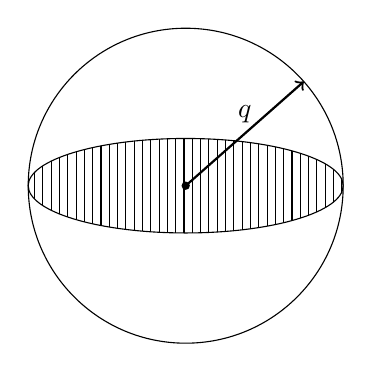
\begin{tikzpicture}
        \draw (0,0) circle (2cm);
        \draw (-2,0) arc (180:360:2 and 0.6) -- (2,0) arc (0:180:2 and 0.6);
        \fill[pattern=vertical lines] (-2,0) arc (180:360:2 and 0.6) -- (2,0) arc (0:180:2 and 0.6);
        \fill (0,0) circle (1.5pt);
        \draw[->, thick] (0,0) -- node[above]{$q$} (1.5,1.323);
    \end{tikzpicture}
    \caption{A 3-dimensional representation of quaternions. \cite{Penguin}}
    \label{SphereQuaternionRepresentation}
\end{figure}

\begin{figure}[ht]
    \centering
    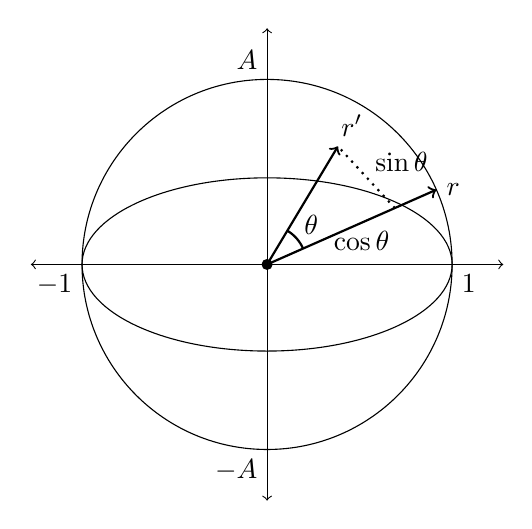
\begin{tikzpicture}
        \draw (0,0) coordinate (A) circle (2.35cm);
        \draw (-2.35,0) arc (180:360:2.35 and 1.1) -- (2.35,0) arc (0:180:2.35 and 1.1);
        \fill (0,0) circle (2pt);

        \draw[<->] (0,-3) -- (0,3);
        \draw[<->] (-3,0) -- (3,0);

        \draw (0,2.35) node[anchor=south east]{$A$};
        \draw (0,-2.35) node[anchor=north east]{$-A$};
        \draw (2.35,0) node[anchor=north west]{$1$};
        \draw (-2.35,0) node[anchor=north east]{$-1$};

        \draw[->, thick] (0,0) -- (0.9,1.5) node[above]{$\quad r'$};
        \draw[->, thick] (0,0) -- (2.15,0.949) node[right]{$r$};

        \draw[dotted, thick] (1.623,0.716) coordinate (B) -- (0.9,1.5) coordinate (C);
        \node[anchor=north] at (1.2,0.55) {$\cos\theta$};
        \node[anchor=west] at (1.25,1.3) {$\sin\theta$};

        \draw pic["$\theta$", draw, thick, angle eccentricity=1.5] {angle = B--A--C};
    \end{tikzpicture}
    \caption{4-dimensional rotations viewed on a unit sphere.}
    \label{4DRotationsLike2DFig}
\end{figure}

In this representation, the $\vb{i,j,k}$ space is thought of as one component, perpendicular to the real numbers. Considering the $\vb{i,j,k}$ space as defining the axis we are rotating around (in the same way that pure quaternions represent vectors - Section \ref{PureDef}), that axis will also be perpendicular to the real numbers, by definition of the orthogonality of the four quaternion components.

We can therefore think of a new diagram, Figure \ref{4DRotationsLike2DFig}, similar to Figure \ref{ComplexRotationFig}, but with the axis perpendicular to the real numbers being the chosen axis to rotate around, instead of $\vb{i}$. This rotation axis, $A$, can be represented as a pure, unit quaternion, where:
\begin{equation}
    A = x\vb{i} + y\vb{j} + z\vb{k}, \quad\quad
    \sqrt{x^2 + y^2 + z^2} = 1, \quad\quad
    x, y, z \in \mathbb{R}.
\end{equation}

Figure \ref{4DRotationsLike2DFig} shows diagrammatically how the same method can be used for quaternion rotations as with 2-dimensional complex number rotations, but with a rotation around the axis $A$ instead of around the origin. While in this diagram $\abs{r} = 1$, as mentioned in Section \ref{qrqIntro}, this is not necessary.

To rotate $r$ to $r'$, just like with complex numbers, $r'$ can be considered to be the sum of two "vectors" (technically quaternions in this 4-dimensional space): the proportion of $r$ in the direction of (parallel to) $r$, and the proportion of $r$ perpendicular to $r$. As shown by the right-angled triangle formed in the diagram (and explained more thoroughly in Section \ref{Complex2DRotation} with complex numbers), the vector parallel to $r$ is $r\cos\theta$, and the vector perpendicular to it is $Ar\sin\theta$. Here, $A$ is used instead of $\vb{i}$, as it is being thought of as the perpendicular axis to the real numbers. Therefore, we can write $r'$ (the rotated point) as:
\footnotetext[1]{This is not fully accurate, but should be considered so for the time being. The true form will be explained in Section \ref{QBarSection}.}
\begin{equation}
    \begin{aligned}
        r' &= r\cos\theta + Ar\sin\theta \\
           &= (\cos\theta + A\sin\theta)r \\
           &= (\cos\theta + (x\vb{i} + y\vb{j} + z\vb{k})\sin\theta)r \\
           &= qr. \footnotemark[1] \\
        \implies q &= \cos\theta + (x\vb{i} + y\vb{j} + z\vb{k})\sin\theta,\footnotemark[1]
    \end{aligned}
\end{equation}
where $q$ is the quaternion that $r$ (a point being rotated in pure quaternion form) is multiplied by for a rotation of $\theta$ radians around the axis $A$.

Since $A$ is a (pure) unit quaternion (which implies $x^2 + y^2 + z^2 = 1$), and $\sin^2\theta + \cos^2\theta \equiv 1$, this will guarantee that $q$ will be a unit quaternion too, as desired:
\begin{equation}
    \begin{aligned}
        \abs{q} &= \sqrt{\cos^2\theta + (x\sin\theta)^2 + (y\sin\theta)^2 + (x\sin\theta)^2} \\
                &= \sqrt{\cos^2\theta + \sin^2\theta(x^2 + y^2 + z^2)} \\
                &= \sqrt{\cos^2\theta + \sin^2\theta} \\
                &= 1.
    \end{aligned}
\end{equation}

The use of sine for the imaginary axis of rotation and cosine for the real component can also be shown by looking at the sine and cosine functions themselves. For an angle of 0 (or any multiple of $2\pi$ - any full rotation), sine and cosine output 0 and 1 respectively. When the angle of rotation, $\theta$, is 0, the desired effect is that $qr$ yields $r$. If sine and cosine are used as given:
\begin{equation}
    r' = qr\footnotemark[1] = (\cos\theta + (x\vb{i} + y\vb{j} + z\vb{k})\sin\theta)r = 1r = r,
\end{equation}
as desired. However, if the roles of sine and cosine were reversed, when $\theta = 0$:
\begin{equation}
    r' = qr\footnotemark[1] = (\sin\theta + (x\vb{i} + y\vb{j} + z\vb{k})\cos\theta)r = (x\vb{i} + y\vb{j} + z\vb{k})r.
\end{equation}
This yields the product of $r$ and axis of rotation, instead of just $r$ as desired. Generalising, it is clear that (in the first quadrant) increasing $\theta$ increases $\sin\theta$ and decreases $\cos\theta$, and the "aim" when rotating is that increasing theta (in the first quadrant) should decrease the parallel (unchanged) component of $r$ and increase the its perpendicular (rotated) component as a proportion of $r'$. This is also clear when looking at Figure \ref{4DRotationsLike2DFig}. Therefore, it is logical that cosine should be used for the real component, and sine for the imaginary rotation axis.

However, there is a problem with the definition of a quaternion rotation above. In fact, $r' \neq qr, r' = qr\bar{q}$, as stated in Section \ref{qrqIntro}. The following section will explain the reason for this, and how the formula above should be changed to reflect this.

\subsection{The purpose of $\bar{q}$} \label{QBarSection}

While it is true, as shown above, that a multiplication by $qr$ rotates $r$ by $\theta$ radians around the axis, $A$, defined by $q$, it also performs a second, undesired, rotation, parallel to $A$. This is best demonstrated through a stereographic projection. \cite{Penguin} \cite{3Blue1Brown}

\begin{figure}[ht]
    \centering
    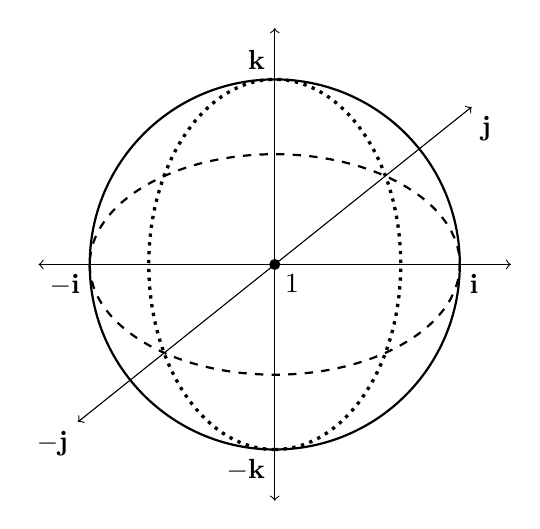
\begin{tikzpicture}
        \draw[thick] (0,0) node[anchor=north west]{$1$} coordinate (A) circle (2.35cm);
        \draw[dashed, thick] (-2.35,0) arc (180:360:2.35 and 1.4) -- (2.35,0) arc (0:180:2.35 and 1.4);
        \fill (0,0) circle (2pt);

        \draw[dotted, very thick] (0,-2.35) arc (-90:90:1.6 and 2.35) -- (0,2.35) arc (90:270:1.6 and 2.35);

        \draw[<->] (0,-3) -- (0,3);
        \draw[<->] (-3,0) -- (3,0);
        \draw[<->] (-2.5,-2) -- (2.5,2);

        \draw (0,2.35) node[anchor=south east]{$\vb{k}$};
        \draw (0,-2.35) node[anchor=north east]{$-\vb{k}$};
        \draw (2.35,0) node[anchor=north west]{$\vb{i}$};
        \draw (-2.35,0) node[anchor=north east]{$-\vb{i}$};
        \draw (-2.5,-2) node[anchor=north east]{$-\vb{j}$};
        \draw (2.5,2) node[anchor=north west]{$\vb{j}$};
    \end{tikzpicture}
    \caption{A stereographic projection of unit quaternions in 3-dimensional space. \cite{Penguin}}
    \label{StereographicFig}
\end{figure}

This stereographic projection (shown in Figure \ref{StereographicFig}) maps every unit quaternion onto a point within 3-dimensional space. Note that the origin represents 1: the unit quaternion with real component 1 and therefore no imaginary component. The edge of this sphere that has been drawn represents every unit quaternion with a real component 0 (i.e. all the pure unit quaternions). The space inside the sphere represents quaternions with real component between 1 and 0, and the space outside the sphere represents the quaternions with negative real components. As a quaternion's real component tends towards -1, its representation in this diagram tends towards being infinitely displaced from the centre.

We are looking to rotate 3-dimensional points, that are represented as pure quaternions, and as such these points will all lie on the edge of the sphere, so we can place our focus on that part of the diagram. Although the quaternion being rotated does not need to be a unit quaternion, this diagram does not represent quaternions with any other magnitude, so the explanations will assume the point being rotated has magnitude 1. However, the explanations will still be relevant for any other pure quaternion, and the diagram can be modified to show quaternions of any magnitude by multiplying each component in the diagram by the desired magnitude. For example, for a magnitude of 2, on the diagram: $1 \rightarrow 2, -\vb{i} \rightarrow -2\vb{i}$, etc.

We can now imagine some multiplications of quaternions using this diagram. If we consider all the points on the sphere to have been left-multiplied by $\vb{i}$ (note the importance of the order of multiplication due to the non-commutativity of quaternion multiplication), using the multiplicative rules $\vb{ij} = \vb{k}$ and $\vb{ik} = -\vb{j}$ (Equation \ref{MultProperties1}, Section \ref{ijkComponentsSection}), we can deduce that the point at $\vb{k}$ will be mapped to the point at $-\vb{j}$, the point at $-\vb{j}$ to $-\vb{k}$, the point at $-\vb{k}$ to $\vb{j}$, and finally the point at $\vb{j}$ to $\vb{k}$. On the diagram (Figure \ref{StereographicFig}), this looks like an anticlockwise rotation on the dotted circle that connects the $\vb{k}$ and $\vb{j}$ axes.

Until this point, there have been no undesired effects - multiplying by $\vb{i}$ has resulted in a rotation perpendicular to, so around, the $\vb{i}$ axis, as desired. However, left-multiplying by $\vb{i}$ also causes a second transformation: one that is parallel to the $\vb{i}$ axis. More generally, a multiplication by any axis, $A$, causes a second rotation parallel to the axis. This can clearly be seen in the diagram, where left-multiplying by $\vb{i}$ also maps $\vb{i}$ to $-1$, $-1$ to $-\vb{i}$, $-\vb{i}$ to 1, and 1 to $\vb{i}$. While -1 cannot be explicitly seen in the diagram, it is the point of infinite distance from the centre of the unit circle, and so this rotation can be considered to "wrap-around" the diagram in a fourth dimension that we do not have access to. Figure \ref{LeftMultIFig} shows a visualisation of this. The arrows indicate the direction of motion upon left-multiplication by $\vb{i}$.

\begin{figure}[H]
    \centering
    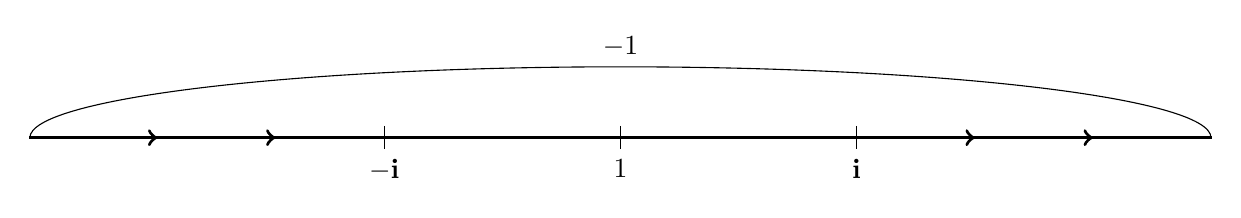
\begin{tikzpicture}[scale=1.5]
        \draw[>->, very thick] (-4,0) -- (4,0);
        \draw[-, very thick] (-5.0047,0) -- (5.0047,0);
        \draw[>->, very thick] (-3,0) -- (3,0);
        \draw (-5,0) arc (180:360:5 and -0.6);
        \node[anchor=south] at (0,0.6) {$-1$};
        \draw (-2,0.1) -- + (0, -0.2) node[below] {$-\vb{i}$};
        \draw (2,0.1) -- + (0, -0.2) node[below] {$\vb{i}$};
        \draw (0,0.1) -- + (0, -0.2) node[below] {$1$};
    \end{tikzpicture}
    \caption{A representation of the theoretical position of -1 in Figure \ref{StereographicFig}.}
    \label{LeftMultIFig}
\end{figure}

The same two rotations (both perpendicular and parallel to the axis) will occur with any axis of rotation, $A$, not necessarily just $\vb{i}$ or a single imaginary component. This behaviour is undesired, as the each multiplication should represent exactly one rotation around one axis. Therefore, the solution is to multiply the current expression, $qr$, by a third component, that will cancel out the rotation parallel to the axis, but not affect the rotation around it. Right-multiplying by $\bar{q}$ has this effect. Using the definition of $\bar{q}$ in Section \ref{qBarDef}:
\begin{equation}
    \begin{aligned}
        q &= a + b\vb{i} + c\vb{j} + d\vb{k} \\
          &= \cos\theta + (b\vb{i} + c\vb{j} + d\vb{k})\sin\theta \\
        \implies \bar{q} &= a - b\vb{i} - c\vb{j} - d\vb{k} \\
          &= \cos\theta - (b\vb{i} + c\vb{j} + d\vb{k})\sin\theta.
    \end{aligned}
\end{equation}
To explain why right-multiplying by $\bar{q}$ has this effect, it is important to consider the implications of the non-commutativity of quaternion rotation: while the product of two different imaginary quaternion components differs based on the order of multiplication, this is not the case when a real number is involved in the multiplication (think of this as the real number "scaling" the imaginary component, rather than changing the axis on which it lies), or when one component is multiplied by itself (e.g. $\vb{i}\times\vb{i} = \vb{i}\times\vb{i}$).

If we consider $qr$ as one point (as it is the pure quaternion formed following the first rotation of $r$), we can then consider the product of $\bar{q}$ with this pure quaternion $qr$. A left-multiplication by $\bar{q}$ would completely cancel out the effect of $q$, since $\bar{q}q$ = 1 (Section \ref{qBarDef}) and quaternion multiplication is associative, i.e. $(\bar{q}q)r = \bar{q}(qr)$. Interpreting this through the stereographic visualisation of unit quaternions, left-multiplying $qr$ by $\bar{q}$ would cause a rotation both parallel and perpendicular to the axis of rotation, opposite but equal in magnitude to the rotation a left-multiplication by $q$ caused. More simply, a left-multiplication of $qr$ by $\bar{q}$ yields $r$, cancelling out the effect of $q$.

The desired multiplication is one that does not affect the rotation perpendicular to the rotation axis, but causes a rotation with the opposite effect to the rotation parallel to it, in effect cancelling out the second, undesired, rotational effect of $q$. Right-multiplying by $\bar{q}$ has a similar effect to this. Since the non-commutativity of quaternion multiplication does not apply to multiplications of the same component, or to multiplications including a real number as one of the numbers being multiplied, this will have the same effect on the parallel axis as when left-multiplying by $\bar{q}$: one that cancels out the effect of $q$ in this axis, as desired. This can be demonstrated with the previous example where the quaternions of multiplication, $q$, is $\vb{i}$. $q=\vb{i}\implies\bar{q}=-\vb{i}$, and right-multiplication by $\vb{i}$ maps $\vb{i}$ to $-1$, $-1$ to $-\vb{i}$, $-\vb{i}$, to 1, and 1 to $\vb{i}$, the exact opposite effect of left-multiplying by $q$, cancelling out this unwanted transformation.

However, the key here is how it affects the desired rotation, the rotation perpendicular to (around) the axis of rotation. In this case, the non-commutativity of multiplying different imaginary quaternion components in relevant, and so right-multiplying by $\vb{-i}$ causes a flip in the sign of the transformations created when compared to left-multiplying by $-\vb{i}$. This means that the theoretical circle between the $\vb{j}$ and $\vb{k}$ axes is rotated in the same direction as when it was left-multiplied by $\vb{i}$, mapping $\vb{k}$ to $-\vb{j}$, $-\vb{j}$ to $-\vb{k}$, $-\vb{k}$ to $\vb{j}$, and $\vb{j}$ to $\vb{k}$ on the stereographic projection. Again, this is the case with any axis, $A$, and so any rotation quaternion, $q$, but the transformation of points with the stereographic projection is simpler to visualise when a whole imaginary component is used as the axis of rotation.

While this right multiplication by $\bar{q}$, forming a final rotation expression of $r' = qr\bar{q}$, cancels out the undesired rotation $q$ causes parallel to the axis of rotation, it does not leave the desired rotation perpendicular to (around) the axis untouched. It instead performs an identical rotation to $q$ around the axis, in effect doubling the rotational effect of the expression. Therefore, defining $q$ as $q = \cos\theta + (A)\sin\theta$ would actually rotate the point, $r$, $2\theta$, not $\theta$, radians around the axis, $A$.

Therefore, we need to redefine $q$ as:
\begin{equation}
    q = \cos\frac{\theta}{2} + A\sin\frac{\theta}{2},
\end{equation}
where $qr\bar{q}$ defines the new position of $r$, a 3-dimensional point in pure quaternion form, when it is rotated $\theta$ radians around the axis, $A$, expressed as a pure unit quaternion.

\subsection{The desirable properties of quaternions}

While the field of quaternions was first defined by Hamilton, in 1843, it was not widely adopted as the standard for defining 3-dimensional geometry, and has only recently come into popularity, with the rise of computers, and the need for efficient computation. \cite{3Blue1Brown}

Euler angles are a key alternative to quaternions for representing 3-dimensional rotations. They work by defining the angle of rotation around each of the $x, y$, and $z$ axes, and the order in which these rotations occur. They are typically much easier to visualise and intuitively understand than quaternions, however, are much less efficient and practical in a computational sense. The reasons for this become clear in this section, as the desirable properties of quaternions are explored.

\subsubsection{The combination of multiple rotations} \label{RotComb}

While there is a need to separately calculate three rotations around separate axes using Euler angles, one quaternion is sufficient to represent any possible 3-dimensional rotation. In fact, due to the non-commutativity of quaternion multiplication (Section \ref{ComAss}), separate rotation quaternions can be multiplied together in their order of rotation to form one quaternion, representing the full rotation, by modifying the axis and angle of rotation accordingly.

This is particularly useful when converting from Euler angles to quaternions. This is a good way of increasing the ease-of-use of rotation systems, such as in a game engine, by allowing the programmer to define a rotation with Euler angles, but allowing the computer to calculate the rotation using quaternions.

For example, given Euler angles of $\frac{\pi}{4}$ radians in the $y$ axis, $\frac{\pi}{2}$ in the $x$ axis, and $-\frac{\pi}{4}$ in the $z$ axis, where rotation is defined in the order $y, x, z$, the resultant quaternion of rotation, $q_r$, can be calculated as follows:
\begin{equation}
    \begin{aligned}
        q &= \cos\frac{\theta}{2}+ (x\vb{i} + y\vb{j} + z\vb{k})\sin\frac{\theta}{2} \\
        q_r &= q_yq_xq_z \\
        \implies q_y &= \cos\frac{\pi}{8} + \sin\frac{\pi}{8}\vb{j} \\
        q_x &= \cos\frac{\pi}{4} + \sin\frac{\pi}{4}\vb{i} \\
        q_z &= \cos-\frac{\pi}{8} + \sin-\frac{\pi}{8}\vb{k} \\
        \implies q_r &= (\cos\frac{\pi}{8} + \sin\frac{\pi}{8}\vb{j})(\cos\frac{\pi}{4} + \sin\frac{\pi}{4}\vb{i})(\cos-\frac{\pi}{8} + \sin-\frac{\pi}{8}\vb{k}) \\
                     &= \frac{1}{2} + \frac{1}{2}\vb{i} + \frac{1}{2}\vb{j} - \frac{1}{2}\vb{k} \\
                     &\phantom{= } \text {after expansion and simplification.}
    \end{aligned}
\end{equation}
Do note here that while we can represent a rotation quaternion as $\cos\theta + (x\vb{i} + y\vb{j} + z\vb{k})\sin\theta$, this is only to allow a better mathematical understanding of the meaning behind the quaternion. In a purely computational sense, the quaternions are stored as four real numbers (one for the real component, and the other three as coefficients of the imaginary components), so trigonometric ratios do not need to be evaluated when calculating rotations with the quaternions produced.

This ability to combine individual rotations into one quaternion vastly reduces the number of calculations that need to be evaluated, and also reduces the possibility of numerical errors, which accumulate with each rotation, due to the computers not storing perfectly precise values for each component.

\subsubsection{Animations}

Another benefit of being able to use one quaternion for any rotation occurs when transitioning between two rotational states of an object. Quaternions make this simple, since the new rotation of the object can simply be calculated by using a fractional multiple of the same $q$ (much more complicated algorithms for more realistic transitions do exist, but use the same principle).

For example, for an animation of a point with $n$ frames, with $r_n$ representing the position of the point in each frame, and $r_0$ its initial position, the frames would be calculated as:
\begin{equation}
    \begin{aligned}
        r_1 &= \frac{1}{n}qr_0\bar{q} \\
        r_2 &= \frac{2}{n}qr_0\bar{q} \\
        ... \\
        r_n &= \frac{n}{n}qr_0\bar{q} = qr_0\bar{q}.
    \end{aligned}
\end{equation}

Note that to rotate a 3-dimensional object, such as a cube, relative to itself, the centre of the object should be considered the origin, and the rotations of each vertex calculated around that.

It is clear how this would be much more difficult with Euler angles, since rotations are defined in terms of three separate motions around separate axes. However, the main benefit of using quaternions here, is that no complex trigonometric ratios need to be evaluated once $q$ has been found: evaluating $qr\bar{q}$ simply requires the addition and multiplication of real numbers, which is much less computationally complex. This is in contrast to Euler angles, where trigonometric ratios would need to be evaluated for every frame, as they are the basis upon which rotation is calculated, which would be very computationally demanding.

\subsubsection{A full example}

While expanding the expression $qr\bar{q}$ by hand can be very time-consuming, with many distributions and simplifications of imaginary quaternion components based upon their defined multiplicative rules, a computer does not need to calculate that for each rotation. After expanding and simplifying the general expression for $qr\bar{q}$ once, the result can be used as a formula for calculating rotations efficiently:
\begin{equation}
    \begin{aligned}
        r' &= qr\bar{q} \\
           &= (a + b\vb{i} + c\vb{j} + d\vb{k})(x\vb{i} + y\vb{j} + z\vb{k})(a - b\vb{i} - c\vb{j} - d\vb{k}) \\
           &= ((a^2 + b^2 - c^2 - d^2)x + 2(bc-ad)y+2(ac+bd)z)\vb{i} \\
           &\phantom{= } + (2(ad+bc)x + (a^2 - b^2 + c^2 - d^2)y + 2(cd-ab)z)\vb{j} \\
           &\phantom{= } + (2(bd-ac)x + 2(ab+cd)y + (a^2 - b^2 - c^2 + d^2)z)\vb{k} \\
           &\phantom{= } \text{after much expansion and simplification.}
    \end{aligned}
\end{equation}

Using the quaternion from Section \ref{RotComb}, $q = \frac{1}{2} + \frac{1}{2}\vb{i} + \frac{1}{2}\vb{j} - \frac{1}{2}\vb{k}$, we can let $a = \frac{1}{2}, b = \frac{1}{2}, c = \frac{1}{2}, d = -\frac{1}{2}$. Assuming we are rotating the point $(1,1,1)$, we can also let $x = 1, y = 1, z = 1$. Substituting these values into the equation, all it takes is a few multiplications and additions to arrive at $r' = \vb{i} - \vb{j} - \vb{k}$. Therefore, the rotated point has co-ordinates $(1, -1, -1)$.

\printbibliography

\end{document}
